\documentclass[a4paper]{article}

\usepackage{amsfonts}
\usepackage{amsmath}
\usepackage[dvips]{epsfig}
\usepackage{dcolumn}
\usepackage{shortvrb}
\usepackage{parskip}
\usepackage{multicol}
\usepackage[dcu]{harvard}

\sloppy
\parindent0em
\topmargin-1.5cm \textheight23cm \textwidth15cm
\oddsidemargin0.5cm

\MakeShortVerb{\|}

\begin{document}

\title{Bayesian Semiparametric Regression Based on Mixed Model Methodology: A Tutorial}
\author{Thomas Kneib, Stefan Lang and Andreas Brezger\\ [.25cm]
\normalsize Department of Statistics, University of Munich. } \maketitle

\begin{abstract}
This tutorial demonstrates the usage of {\it BayesX} for analysing Bayesian semiparametric regression models based on mixed
model methodology. As an example, we consider data on undernutrition of children in Zambia. The tutorial is designed to be
self-contained and describes all features of {\it BayesX} in detail, that will be needed throughout the tutorial. Therefore it
may also serve as a first introduction into the general usage of {\it BayesX}. Note that the tutorial is written for the
version of {\it BayesX} including a graphical user interface and graphics facilities. While all regression-related commands can
be executed in the command line version as well, the graphics facilities will not be available.
\end{abstract}

\tableofcontents

\newpage

\section{Introduction}\label{reml:data}

This tutorial demonstrates the usage of {\it BayesX} for analysing Bayesian semiparametric regression models based on mixed
model methodology. As an example, we consider data on childhood undernutrition in Zambia. This data has already been analysed
in \citeasnoun{kanlan01} and we will use the same model that has been developed there. Since our focus is on demonstrating how
regression models can be estimated in {\it BayesX}, we do not discuss or interpret the estimation results but simply give the
commands to obtain them.

The main focus in this tutorial is on empirical Bayes inference based on mixed model methodology. {\it BayesX} also supports
two further inferential concepts: full Bayesian inference based on MCMC and a method for simultaneously selecting variables and
smoothing parameters, which are described in two additional tutorials. All tutorials are designed to be self-contained and
describe all features of {\it BayesX} in detail, that will be needed throughout the tutorial. Users who are already familiar
with the usage of {\it dataset} and {\it map objects} may therefore skim through sections \ref{reml:usage}--\ref{reml:maps}.

The theoretical background of Bayesian semiparametric regression will not be described in this tutorial. The reference manual
may serve as a first introduction, while further details about the estimation techniques for the empirical Bayes approach in
the context of univariate exponential families can be found in \citeasnoun{fahkne04}. Categorical extensions are treated in
\citeasnoun{kneib2006a} while \citeasnoun{kneib2006b} and \citeasnoun{kneib2007} deal with the analysis of continuous time
survival analysis.

\section{Description of the data set}

Undernutrition among children is usually determined by assessing an anthropometric status of the children relative to a
reference standard. In our example, undernutrition is measured by stunting or insufficient height for age, indicating chronic
undernutrition. Stunting for a child $i$ is determined using a Z-score defined as
\[
Z_i = \frac{AI_i-MAI}{\sigma}
\]
where $AI$ refers to the child`s anthropometric indicator (height at a certain age in our example), while MAI and $\sigma$
correspond to the median and the standard deviation in the reference population, respectively.

Our main interest is on modelling the dependence of undernutrition on covariates including the age of the child, the body mass
index of the child`s mother, the district the child lives in and some further categorial covariates. Table \ref{reml:zambiavar}
gives a description of the variables that we will use in our model.

{\footnotesize
\begin{table}[ht]
\begin{center}
\begin{tabular}{lp{12.5cm}}
 \hline
 {\bf Variable} & {\bf Description}\\
 \hline
 $\mathit hazstd$ & standardised Z-score for stunting\\
 $\mathit bmi$ & body mass index of the mother\\
 $\mathit agc$ & age of the child in months\\
 $\mathit district$ & district where the mother lives\\
 $\mathit rcw$ & mother`s employment status with categories ``working'' (= 1) and ``not working'' (= $-1$)\\
 $\mathit edu1/2$ & mother`s educational status with categories ``complete primary but incomplete secondary'' ($edu1=1$), ``complete secondary or higher'' ($edu2=1$) and ``no education or incomplete primary'' ($edu1=edu2=-1$)\\
 $\mathit tpr$ & locality of the domicile with categories ``urban'' (= 1) and ``rural'' (= $-1$)\\
 $\mathit sex$ & gender of the child with categories ``male'' (= 1) and  ``female'' (= $-1$)\\
 \hline
\end{tabular}
{\it\caption{Variables in the undernutrition data set. \label{reml:zambiavar}}}
\end{center}
\end{table}}

\section{Getting started}\label{reml:usage}

After having started the graphical user interface version of {\it BayesX}, a main window with four sub-windows appears on the
screen. These are the {\it command window} for entering and executing code, the {\it output window} for displaying results, the
{\it review window} for easy access to past commands, and the {\it object browser} that displays all objects currently
available. In the command line version of {\it BayesX}, there are, of course, no sub-windows but only command line prompt to
enter commands.

{\it BayesX} is object oriented although the concept is limited, i.e. inheritance and other concepts of object oriented
languages like C++ or R are not supported. For every object type, a number of object-specific methods can be applied to a
particular object instance. The syntax for generating a new object in {\it BayesX} is

{\tt> }{\it objecttype objectname}

where {\it objecttype} defines the type of the object to be created, e.g. {\tt dataset}, and {\it objectname} is the name to be
assigned to the new object.

The rest of the tutorial is separated in five parts dealing with the different steps of estimating a regression model based on
mixed model methodology. In section \ref{reml:datasets}, we create a {\it dataset object} to store, handle and manipulate the
data. We will also give a brief description of some methods that may be applied to {\it dataset objects}. Since we want to
estimate a spatial effect of the district in which a child lives, we need the boundaries of the districts to compute the
neighbourhood information of the map of Zambia. This information will be stored in a {\it map object}. Section \ref{reml:maps}
describes how to create and handle these objects. Estimation of the regression model is carried out in section
\ref{reml:regression} using a {\it remlreg object}. The last two sections describe how to visualise the estimation results and
how to customise the obtained graphics.

If you have not done so yet, please download the data set and the {\it boundary file} associated with this tutorial now (from
the {\it BayesX} homepage). You may also want to download the batch file containing the commands used in the following
sections. Please note, that paths within these commands must be changed according to the storage location of the corresponding
files on your hard disk.

\section{Reading data set information}\label{reml:datasets}

In a first step, we read the available data set information into {\it BayesX}. Therefore we create a {\it dataset object} named
|d|:

|> dataset d|

We store the data in |d| using the method |infile|:

|> d.infile, maxobs=5000 using c:\data\zambia.raw|

Note, that we assume the data to be provided in the external file |c:\data\zambia.raw|. The first few lines of this file look
like this:

{\footnotesize
 hazstd bmi agc district rcw edu1 edu2 tpr sex\\
 0.0791769 \,\, 21.83 \,\, 4 \,\, 81 \,\, -1 \,\, 1 \,\, 0 \,\, 1 \,\, -1\\
 -0.2541965 \,\, 21.83 \,\, 26 \,\, 81 \,\, -1 \,\, 1 \,\, 0 \,\, 1 \,\, -1\\
 -0.1599823 \,\, 20.43 \,\, 56 \,\, 81 \,\, 1 \,\, -1 \,\, -1 \,\, 1 \,\, 1\\
 0.1733911 \,\, 22.27 \,\, 6 \,\, 81 \,\, -1 \,\, 0 \,\, 1 \,\, 1 \,\, 1}

In our example, the file contains the variable names in the first line. Therefore, it is not necessary to specify them in the
|infile| command. If the file contained only the data without variable names, we would have to supply them after the keyword
|infile|:

 |> d.infile hazstd bmi agc district rcw edu1 edu2 tpr sex, maxobs=5000|
 |  using c:\data\zambia.raw|

Option |maxobs| can be used to speed up the execution time of the |infile| command. If |maxobs| is specified, {\it BayesX}
allocates enough memory to store all the data while the total amount of required memory is unknown in advance if |maxobs|
remains unspecified. For larger data sets, this may cause {\it BayesX} to start reading the data set information several times
because the currently allocated memory is exceeded. However, this is only meaningful for larger data sets with more than 10,000
observations and could therefore be omitted in our example.

A second option that may be added to the |infile| command is the |missing| option to indicate missing values. Specifying for
example |missing = M| defines the letter `|M|' as an indicator for a missing value. The default for missing values are a period
`.' and `|NA|' (which remain valid indicators for missing values even if an additional indicator is defined by the |missing|
option).

After having read the dataset information, we can inspect the data visually. Executing the command

|> d.describe|

opens an {\it Object-Viewer} window containing the data in form of a spreadsheet (see Figure \ref{reml:screenshot}). The same
can also be achieved by double-clicking on the {\it dataset object} in the {\it object browser}.

\vspace{1cm}

\begin{figure}[ht]
\begin{center}
\epsfig{file=grafiken/screenshot2.eps,scale=0.5} {\it\caption{A
screenshot of the dataset.\label{reml:screenshot}}}
\end{center}
\end{figure}

Further methods allow to examine the variables in the {\it dataset object}. For a categorial variable such as $\mathit{sex}$,
the |tabulate| command may be used to produce a frequency table:

|> d.tabulate sex|

resulting in

\begin{verbatim}
Variable: sex

          Value       Obs           Freq            Cum
             -1      2451         0.5057         0.5057
              1      2396         0.4943              1
\end{verbatim}

being printed in the {\it output window}. For continuous variables,  the |descriptive| command prints several characteristics
of the variable in the {output window}. E.g., executing

|> d.descriptive bmi|

leads to

\begin{verbatim}
   Variable    Obs        Mean      Median         Std         Min         Max
        bmi   4847   21.944349        21.4   3.2879659        12.8       39.29
\end{verbatim}

\section{Map objects}\label{reml:maps}

In the following, we will estimate a spatially correlated effect of the district in which a child lives. Therefore we need the
boundaries of the districts in Zambia to compute the neighbourhood information of the map of Zambia. We therefore create a {\it
map object}

|> map m|

and read the boundaries using the |infile| command of {\it map objects}:

|> m.infile using c:\data\zambia.bnd|

Having read the boundary information, {\it BayesX} automatically computes the neighbourhood matrix of the map.

The file following the keyword |using| is assumed to contain the boundaries in form of closed polygons. To give an example we
print a small part of the boundary file of Zambia. The map corresponding to the section of the boundary file can be found in
Figure \ref{reml:zambia52}.

\footnotesize

\hspace{1cm}  $\vdots$

 "52",48\\
 28.080507,-12.537530\\
 28.083376,-12.546980\\
 28.109501,-12.548961\\
 28.134972,-12.566787\\
 28.154797,-12.585320\\
 28.165771,-12.593912\\
 28.165771,-12.593912\\
 28.160769,-12.609917\\
 28.152800,-12.633824\\
 28.144831,-12.657733\\
 28.132877,-12.677656\\
 28.120922,-12.701565\\
 28.120922,-12.717505\\
 28.120922,-12.741411\\
 28.116938,-12.761335\\
 28.108969,-12.777274\\
 28.100998,-12.793213\\
 28.089045,-12.817122\\
 28.085060,-12.837045\\
 28.081076,-12.856968\\
 28.081076,-12.876892\\
 28.080862,-12.884153\\
 28.080862,-12.884153\\
 28.076630,-12.879521\\
 28.031454,-12.881046\\
 27.974281,-12.884675\\
 27.910725,-12.878692\\
 27.686228,-12.880120\\
 27.665676,-12.854732\\
 27.653563,-12.818301\\
 27.639263,-12.759848\\
 27.648254,-12.699927\\
 27.662464,-12.680613\\
 27.662464,-12.680613\\
 27.666534,-12.675080\\
 27.703260,-12.679779\\
 27.752020,-12.695455\\
 27.797932,-12.702188\\
 27.836775,-12.707567\\
 27.867813,-12.699892\\
 27.902308,-12.667418\\
 27.922668,-12.630853\\
 27.943035,-12.596350\\
 27.963434,-12.571486\\
 27.983179,-12.563844\\
 28.016331,-12.554779\\
 28.070650,-12.542199\\
 28.080507,-12.537530\\

\hspace{1cm} $\vdots$

\normalsize

\vspace{0.3cm}

For each region of the map, the boundary file must contain the identifying name of the region, the polygons that form the
boundary of the region, and the number of lines the polygon consists of. The first line always contains the region code
surrounded by quotation marks and the number of lines the polygon of the region consists of. The code and the number of lines
must be separated by a comma. The subsequent lines contain the coordinates of the straight lines that form the boundary of the
region. The straight lines are represented by the coordinates of their end points. Coordinates must be separated by a comma.
Note that the first and the last point must be identical (see the example above) to obtain a closed polygon. Compare chapter 5
of the reference manual for a detailed description of some special cases, e.g. regions divided into subregions.

\begin{figure}[h]
\centering

\includegraphics [scale=0.3]{grafiken/zambia52.ps}
\caption{\label{reml:zambia52} Corresponding graph of the section of
the boundary file}
\end{figure}

{\it Map objects} may be visualised using method |describe|:

|> m.describe|

resulting in the graph shown in Figure \ref{reml:zambiamap}. Additionally, |describe| prints further information about the {\it
map object} in the {\it output window} including the name of the object, the number of regions, the minimum and maximum number
of neighbours and the bandwidth of the corresponding adjacency or neighbourhood matrix:

\begin{verbatim}
  MAP m
  Number of regions: 54
  Minimum number of neighbors: 1
  Maximum number of neighbors: 9
  Bandsize of corresponding adjacency matrix: 24
\end{verbatim}

\begin{figure}[ht]
\begin{center}
\epsfig{file=grafiken/zambia.ps,scale=0.35} {\it\caption{The
districts within Zambia.\label{reml:zambiamap}}}
\end{center}
\end{figure}

Reading the boundary information from an external file and computing the neighbourhood matrix may be a computationally
intensive task if the map contains a large number of regions or if the polygons are given in great detail. To avoid doing these
computation in every {\it BayesX} session, we store the neighbourhood information in a {\it graph file} using method |outfile|
together with the |graph| option:

|> m.outfile, replace graph using c:\data\zambiasort.gra|

A graph file stores the nodes and the edges of a graph $G = (N,E)$, see for example \citeasnoun{geoliu81} for a first
introduction into graph theory. A graph is a convenient way of representing the neighbourhood structure of a geographical map.
The nodes of the graph correspond to the region codes. The neighbourhood structure is represented by the edges of the graph. In
some situations it may be useful to define weights associated with the edges of a graph which can be be stored in the {\it
graph file} as well.

We now describe the structure of a graph file as it is expected by {\it BayesX}. The first line of a {\it graph file} must
contain the total number of nodes of the graph. In the remaining lines, the nodes of the graph together with their edges and
associated weights are specified. One node corresponds to three consecutive lines. The first of the three lines must contain
the name of the node, which typically will be the name of the geographical region. In the second line, the number of edges of
that particular node is given. The third line contains the corresponding edges of the node, where an edge is given by the index
of a neighbouring node. The index starts with zero. For example, if the fourth and the seventh node/region in the {\it graph
file} are connected/neighbours, the edge index for the fourth node/region is 6 and for the seventh node/region 3.

We illustrate the structure of a graph file with an example. The following few lines are the beginning of the graph file
corresponding to the reordered map of Zambia:

\footnotesize

 57\\
 87\\
 1\\
 5\\
 76\\
 3\\
 9 8 7\\
 67\\
 2\\
 10 9\\

\hspace{1cm} $\vdots$

\normalsize

\vspace{0.5cm}

The first line specifies the total number of nodes, in the present example 57 nodes. The subsequent three lines correspond to
the node with name `87', which is the first region in the reordered map of Zambia. Region `87' has 1 neighbour, namely the
sixth node appearing in the graph file. Once again, note that the index starts with zero, i.e. 0 corresponds to the first node,
1 corresponds to the second node and so on. Lines 5 to 7 in the example correspond to node `76' and its three neighbours and
lines 8 to 10 correspond to node `67'.

In a graph file it is also possible to specify weights associated with the edges of the nodes. Since in the preceding example
no weights are explicitly specified, all weights are automatically defined to be equal to one. Nonequal weights are specified
in the graph file by simply adding them following the edges of a particular node. An example of the beginning of a graph file
with weights is given below:

\footnotesize

 57\\
 87\\
 1\\
 5 1.44172\\
 76\\
 3\\
 7 8 9 0.707424 1.3816 0.682372\\
 67\\
 2\\
 9 10 1.67424 0.8406\\

\hspace{1cm} $\vdots$

\normalsize

\vspace{0.5cm}

Here the edge of the first node `87' has weight 1.44172, the edges of the second node have weights 0.707424, 1.3816 and
0.682372.

Note, that graph files allow the estimation of very general correlated effects based on Markov random fields. While the
polygons stored in a {\it boundary file} represent geographical information, the nodes and edges of a graph may define
arbitrary neighbourhood structures. For example, the definition of three-dimensional Markov random fields representing
space-time interactions is possible.

To see how storing maps in {\it graph files} affects the computation time of the |infile| command, we create a second {\it map
object} and read in the information from the graph file. Again, we have to specify the keyword |graph|:

\begin{verbatim}
> map m1
> m1.infile, graph using c:\data\zambiasort.gra
\end{verbatim}

As you should have noticed, reading geographical information from a {\it graph file} is usually much faster than reading from a
{\it boundary file}. However, using {\it graph files} also has a drawback. Since they do no longer contain the full information
on the polygons forming the map, we can not visualise a {\it map object} created from a {\it graph file}. Trying to do so

|> m1.describe|

raises an error message. This implies, that visualising estimation results of spatial effects can only be based on {\it map
objects} created from {\it boundary files}, although estimation can be carried out using {\it graph files}. Since we will work
with the {\it map object} |m| in the following, we delete |m1|:

|> drop m1|

\section{Bayesian semiparametric regression}\label{reml:regression}

To estimate a regression model based on mixed model techniques, we first create a {\it remlreg object}:

|> remlreg r|

By default, estimation results are written to the subdirectory |output| of the installation directory. In this case, the
default filenames are composed of the name of the {\it remlreg object} and the type of the specific file. Usually it is more
convenient to store the results in a user-specified directory. To define this directory we use the |outfile| command of {\it
remlreg objects}:

|> r.outfile = c:\data\r|

Note, that |outfile| does not only specify a directory but also a base filename (the character `r' in our example). Therefore
executing the command above leads to storage of the results in the directory |c:\data| and all file names will start with the
character `r'. Of course the base filename may be different from the name of the {\it remlreg object}.

In addition to parameter estimates, {\it BayesX} also produces some further information on the estimation process. In contrast
to parameter estimates, this information is not stored automatically but is printed in the {\it output window}. Therefore it is
useful to store the contents of the {\it output window}. This can be achieved automatically by opening a {\it log file} using
the |logopen| command

|> logopen, replace using c:\data\logreml.txt|

After opening a {\it log file}, every information written to the output window is also stored in this file. Option |replace|
allows {\it BayesX} to overwrite an existing file with the same name as the specified {\it log file}. Without |replace|,
results are appended to an existing file.

The model presented in \citeasnoun{kanlan01} is given by the following semiparametric predictor:
\[
 \eta=\gamma_0+\gamma_1\mathit{rcw}\gamma_2\mathit{edu1}+\gamma_3\mathit{edu2}+\gamma_4\mathit{tpr}+\gamma_5\mathit{sex}+
 f_1(\mathit{bmi})+f_2(\mathit{agc})+f^{\mathrm{str}}(\mathit{district})+f^{\mathrm{unstr}}(\mathit{district}).
\]
The two continuous covariates {\it bmi} and {\it agc} are assumed to have a possibly nonlinear effect on the Z-score and are
therefore modelled nonparametrically (as P-splines with second order random walk prior in our example). The spatial effect of
the district is split up into a spatially correlated part $f^{\mathrm{str}}(\mathit{district})$ and an uncorrelated part
$f^{\mathrm{unstr}}(\mathit{district})$, see \citeasnoun{fahlan01b} for a motivation. The correlated part is modelled by a
Markov random field prior, where the neighbourhood matrix and possible weights associated with the neighbours are obtained from
the {\it map object} |m|. The uncorrelated part is modelled by an  i.i.d. Gaussian effect.

To estimate the model we use method |regress| of {\it remlreg objects}:
\begin{verbatim}
> r.regress hazstd = rcw + edu1 + edu2 + tpr + sex + bmi(psplinerw2)
  + agc(psplinerw2) + district(spatial,map=m) + district(random),
  family=gaussian lowerlim=0.01 eps=0.0005 using d
\end{verbatim}

Options |lowerlim| and |eps| control the estimation process. Since small variances are near to the boundary of their parameter
space, the usual Fisher-scoring algorithm for their determination has to be modified. If the fraction of the penalised part of
an effect relative to the total effect is less than |lowerlim|, the estimation of the corresponding variance is stopped and the
estimator is defined to be the current value of the variance (see the  reference manual for details). The option |eps| defines
the termination criterion for the estimation process. The default value for |lowerlim| is 0.001, the default value for |eps| is
0.00001. However, since our analysis is only for explanatory purpose, we chose somewhat weaker conditions resulting in a faster
``convergence'' of the algorithm.

A further option of method |regress| is |maxit|, defining the maximum number of iterations that should be performed in the
estimation. Note, that {\it BayesX} produces results based on the current values of all parameters even if no convergence could
be achieved within |maxit| iterations, but a warning message will be printed in the {\it output window}.

In the following we reproduce the content of the {\it output window} to make the user familiar with the estimation results
produced by {\it BayesX}. Note that the output may look somewhat different depending on the version of {\it BayesX} you are
considering.

\footnotesize
\begin{verbatim}
ESTIMATION RESULTS:


  Estimated scale parameter: 0.802145

  Scale parameter is also stored in file
  c:\data\r_scale.res


  f_bmi_pspline


  Estimated variance:  1.14819e-05
  Inverse variance:    87093.8
  Smoothing parameter: 69861.9
  (Smoothing parameter = scale / variance)
  Degrees of freedom: 1.17481
  NOTE: Estimation of the variance was stopped after iteration 6
        because the corresponding penalized part was small relative to the linear predictor.

  Variance and smoothing parameter are stored in file
  c:\data\r_f_bmi_pspline_var.res

  Results are stored in file
  c:\data\r_f_bmi_pspline.res

  Postscript file is stored in file
  c:\data\r_f_bmi_pspline.ps

  Results may be visualized using method 'plotnonp'
  Type for example: objectname.plotnonp 1


  f_agc_pspline


  Estimated variance:  0.00322146
  Inverse variance:    310.418
  Smoothing parameter: 249.001
  (Smoothing parameter = scale / variance)
  Degrees of freedom: 6.19468

  Variance and smoothing parameter are stored in file
  c:\data\r_f_agc_pspline_var.res

  Results are stored in file
  c:\data\r_f_agc_pspline.res

  Postscript file is stored in file
  c:\data\r_f_agc_pspline.ps

  Results may be visualized using method 'plotnonp'
  Type for example: objectname.plotnonp 2

  f_district_spatial


  Estimated variance:  0.0294011
  Inverse variance:    34.0123
  Smoothing parameter: 27.2828
  (Smoothing parameter = scale / variance)
  Degrees of freedom: 16.7629

  Variance and smoothing parameter are stored in file
  c:\data\r_f_district_spatial_var.res

  Results are stored in file
  c:\data\r_f_district_spatial.res

  Postscript file is stored in file
  c:\data\r_f_district_spatial.ps

  Results may be visualized in BayesX using method 'drawmap'
  Type for example: objectname.drawmap 3



  f_district_random


  Estimated variance:  0.00806667
  Inverse variance:    123.967
  Smoothing parameter: 99.4393
  (Smoothing parameter = scale / variance)
  Degrees of freedom: 14.2076

  Variance and smoothing parameter are stored in file
  c:\data\r_f_district_random_var.res

  Results for random effects are stored in file
  c:\data\r_f_district_random.res

  FixedEffects


  Variable  Post. Mode     Std. Dev.      p-value        95% Confidence Interval
  const     0.0610359      0.0341574      0.0734909      -0.00592615    0.127998
  rcw       0.00767163     0.0136563      0.573859       -0.0191002     0.0344435
  edu1      -0.0605106     0.0261369      0.020636       -0.111749      -0.00927198
  edu2      0.234918       0.0459925      8.82492e-06    0.144754       0.325081
  tpr       0.0904094      0.0218891      0.000123529    0.047498       0.133321
  sex       -0.0585716     0.0129304      4.08485e-05    -0.0839203     -0.0332229

  Results for fixed effects are also stored in file
  c:\data\r_FixedEffects.res


  Model Fit


  -2*log-likelihood:                 3733.37
  Degrees of freedom:                44.34
  (conditional) AIC:                 3822.05
  (conditional) BIC:                 4109.65
  GCV:                               0.809435

  Results on the model fit are stored in file
  c:\data\r_modelfit.raw


  Additive predictor and expectations


  Additive predictor and expectation for each observation are stored in file
  c:\data\r_predict.raw

  Files of model summary:

  ---------------------------------------------------------------------------

  Batch file for visualizing effects of nonlinear functions is stored in file
  c:\data\r_graphics.prg

  NOTE: 'input filename' must be substituted by the filename of the boundary-file

  ---------------------------------------------------------------------------

  Batch file for visualizing effects of nonlinear functions
  in R / S-Plus is stored in file
  c:\data\r_r_splus.txt

  NOTE: 'input filename' must be substituted by the filename of the boundary-file

  ---------------------------------------------------------------------------

  Latex file of model summaries is stored in file
  c:\data\r_model_summary.tex

  ---------------------------------------------------------------------------
\end{verbatim}
\normalsize

In addition to the information being printed to the {\it output window}, results for each effect are written to external ASCII
files. The names of these files are given in the output window, compare the previous pages. For the variance parameters, the
files contain the variance as well as the corresponding smoothing parameter and degrees of freedom. For the different terms of
the model, the files contain the posterior mode, the 80\% and 95\% credible interval, the standard deviations and the
corresponding 95\% and 80\% posterior probabilities of the estimated effects (unless other levels have been requested). For
example, the beginning of the file |c:\data\r_f_bmi_pspline.res| for the effect of {\it bmi} may look like this:

{\footnotesize
 intnr \,\, bmi \,\, pmode \,\, ci95lower \,\, ci80lower \,\, std \,\, ci80upper \,\, ci95upper \,\, pcat95 \,\, pcat80\\
 1 \,\, 12.8 \,\, -0.22305 \,\, -0.304661 \,\, -0.276409 \,\, 0.0416301 \,\, -0.169692 \,\, -0.141439 \,\, -1 \,\, -1\\
 2 \,\, 13.15 \,\, -0.215246 \,\, -0.292828 \,\, -0.26597 \,\, 0.0395749 \,\, -0.164522 \,\, -0.137663 \,\, -1 \,\, -1\\
 3 \,\, 14.01 \,\, -0.19607 \,\, -0.264173 \,\, -0.240597 \,\, 0.0347394 \,\, -0.151544 \,\, -0.127968 \,\, -1 \,\, -1\\}

The credible intervals and posterior probabilities that are computed for every effect may be changed by the user via the
options |level1| and |level2|. For example, specifying |level1=99| and |level2=70| in the option list of the |regress| command
leads to the computation of 70\% and 99\% credible intervals and posterior probabilities. The defaults are |level1=95| and
|level2=80|.

Some nonparametric effects are visualised by {\it BayesX} automatically and the resulting graphs are stored in ps format. For
example, the effect of $\mathit{bmi}$ is visualised in the file |c:\data\b_f_bmi_pspline.ps| (compare the results on the
previous pages for the other filenames). A batch file to reproduce the plots is stored in the output directory. In our example
the name of the file is |c:\data\r_graphics.prg|. The advantage is that additional options may be added by the user to
customise the graphs (compare the following two sections).

Moreover, a file with ending |.tex| is created in the outfile directory. This file contains a summary of the estimation results
and may be compiled using \LaTeX.

Having finished the estimation, we may close the {\it log file} by typing

|> logclose|

Note, that the {\it log file} is closed automatically when you exit {\it BayesX}.

\section{Visualising estimation results}\label{reml:visual}

{\it BayesX} provides three possibilities to visualise estimation results:
\begin{itemize}
\item As mentioned in the previous section, certain results are automatically visualised by {\it BayesX} and stored in {\it
    ps files}.
\item Post estimation commands of {\it remlreg objects} allow to visualise results after having executed a |regress|
    command.
\item {\it Graph objects} may be used to produce graphics using the ASCII files containing the estimation results. In
    principle, {\it graph objects} allow the visualisation of any content of a {\it dataset object}. {\it Graph files} are
    also used in the batch file containing the commands to reproduce the automatically generated graphics.
\end{itemize}

In this section, we describe the general usage of the post estimation commands as well as the commands for the usage with {\it
graph objects} to enable the user to reproduce the automatically generated plots directly in {\it BayesX}. Section
\ref{reml:custom} describes how to customise plots.

\subsection{Post estimation commands}

After having estimated a regression model, plots for nonparametric effects of metrical covariates can be produced using the
post estimation command |plotnonp|:

|> r.plotnonp 1|

and

|> r.plotnonp 2|

produce the graphs shown in Figure \ref{reml:bmi1} in an {\it object-viewer window}. The numbers following the |plotnonp|
command depend on the order in which the model terms have been specified (and an internal ordering of the effect types). The
numbers are supplied in the {\it output window} after estimation, compare the results in the previous section.

By default, the plots contain the posterior mode and pointwise credible intervals according to the levels specified in the
|regress| command. Hence, by default the plots include pointwise 80\% and 95\% credible intervals.

\begin{figure}[ht]
\begin{center}
\epsfig{file=grafiken/zambia_reml_f_bmi1.ps,scale=0.5}
\epsfig{file=grafiken/zambia_reml_f_age1.ps,scale=0.5} {\it\caption{Effect of
the body mass index of the child`s mother and of the age of the
child together with pointwise 80\% and 95\% credible intervals.
\label{reml:bmi1}}}
\end{center}
\end{figure}

A plot may be stored in ps format using the |outfile| option. Executing

|> r.plotnonp 1, replace outfile = c:\data\f_bmi.ps|

stores the plot for the estimated effect of $\mathit{bmi}$ in the file |c:\data\f_bmi.ps|. Again, specifying |replace| allows
{\it BayesX} to overwrite an existing file. Note, that {\it BayesX} does not display the graph on the screen if the option
|outfile| is specified.

Estimation results for spatial effects are best visualised by drawing the respective map and colouring the regions of the map
according to some characteristic of the posterior, e.g. the posterior mode. For the structured spatial effect this can be
achieved using the post estimation command |drawmap|

|> r.drawmap 3|

which results in the graph shown in Figure \ref{reml:spat1}.

\begin{figure}[ht]
\begin{center}
\epsfig{file=grafiken/zambia_reml_f_spat1.ps,scale=0.35}
{\it\caption{Posterior mode of the structured spatial
effect.\label{reml:spat1}}}
\end{center}
\end{figure}


\subsection{Graph Objects}

The commands presented in the previous subsection work only after having estimated a regression model in the current {\it
BayesX} session. However, it may of course also be useful to visualise results of former analyses. This can be achieved using
{\it graph objects}. Note again, that {\it graph files} are also used in the batch file containing the commands to reproduce
the automatically generated graphics. Therefore the purpose of this subsection is also to enable the user to understand the
content of this batch file.

In a first step, we read the estimation results into a {\it dataset object}. For example the estimation results for the effect
of $\mathit{bmi}$ can be read into {\it BayesX} by executing the commands

\begin{verbatim}
> dataset res
> res.infile using c:\data\r_f_bmi_pspline.res
\end{verbatim}

Now the estimation results (or any content of a {\it dataset object}) may be visualised using a {\it graph object} which we
create by typing

|> graph g|

The results stored in the {\it dataset object} |res| are now visualised using the |plot| command of {\it graph objects}.
Executing

 |> g.plot bmi pmode ci95lower ci80lower ci80upper ci95upper using res|

reproduces the graph in Figure \ref{reml:bmi1}.

Similar as for |plotnonp|, the direct usage of the |drawmap| command is only possible after executing a |regress| command.
However, using {\it graph objects} again allows us to visualise results that have been stored in a file.

First we read the information contained in this file into a {\it dataset object}. For example, the following command

|> res.infile using c:\data\r_f_district_spatial.res|

stores the estimation results for the structured spatial effect in the {\it dataset object} |res|. Now we can visualise the
posterior mode using method |drawmap| of {\it graph objects} leading again to the graph shown in Figure \ref{reml:spat1}:

|> g.drawmap pmode district, map=m using res|

Since -- in contrast to a {\it remlreg object} -- no {\it map object} is associated with a {\it graph object} we explicitly
have to specify the map that we want to use in the option list.

Using {\it graph objects} also allows us to plot other characteristics of the posterior than the posterior mode. For instance
the posterior 95\% probabilities may be visualised by

|> g.drawmap pcat95 district, map=m using res|

The result is shown in Figure \ref{reml:spat2}.

\begin{figure}[ht]
\begin{center}
\epsfig{file=grafiken/zambia_reml_f_spat2.ps,scale=0.35}
{\it\caption{Posterior 95\% probability of the structured spatial
effect.\label{reml:spat2}}}
\end{center}
\end{figure}

A further advantage of {\it graph objects} is that they allow to visualise the estimation results for the uncorrelated spatial
effects. Since these are modelled as unstructured random effects, {\it BayesX} is unable to recognise them as spatial effects.
However, proceeding as follows gives us the possibility to plot the unstructured spatial effect shown in Figure
\ref{reml:random1}:

\begin{verbatim}
> res.infile using c:\data\r_f_district_random.res
> g.drawmap pmode district, map=m color swapcolors using res
\end{verbatim}

\begin{figure}[ht]
\begin{center}
\epsfig{file=grafiken/zambia_reml_f_random1.ps,scale=0.35}
{\it\caption{Posterior mode of the unstructured spatial
effect.\label{reml:random1}}}
\end{center}
\end{figure}

\section{Customising graphics}\label{reml:custom}

This section describes how to customise graphics created in {\it BayesX}. All options are described for the usage with the post
estimation commands but may be used with graph files as well. Hence, the options presented in this section also enable the user
to modify the batch file containing the commands to reproduce the automatically generated graphics.

For the presentation of nonparametric effects it may be desirable to include only one of the credible intervals into the plot.
This is achieved by specifying the |levels| option. Possible values of this option are |1| and |2|, corresponding to the levels
specified in the |regress| command (compare section \ref{reml:regression}). If the default values of |level1| and |level2| have
been used, specifying |level=2| in the |plotnonp| command causes {\it BayesX} to plot the 80\% credible interval only (Figure
\ref{reml:bmi3}):

|> r.plotnonp 1, levels=2|

\begin{figure}[ht]
\begin{center}
\epsfig{file=grafiken/zambia_reml_f_bmi3.ps,scale=0.5} {\it\caption{Effect of
the body mass index of the child`s mother with pointwise 80\%
credible intervals only.\label{reml:bmi3}}}
\end{center}
\end{figure}

It may be useful to add some more information to the graphs of nonparametric effects to distinguish more obviously between
different covariates. Ways to do so are the specification of a title or the specification of axis labels. Both possibilities
are supported by {\it BayesX} as demonstrated in the following examples (compare Figure \ref{reml:bmi4} for the resulting
plots):

\begin{verbatim}
> r.plotnonp 1, title="Mother body mass index"
> r.plotnonp 1, xlab="bmi" ylab="f_bmi" title="Mother body mass index"
\end{verbatim}

\begin{figure}[ht]
\begin{center}
\begin{multicols}{2}
\epsfig{file=grafiken/zambia_reml_f_bmi4.ps,scale=0.5}
\epsfig{file=grafiken/zambia_reml_f_bmi5.ps,scale=0.5}
\end{multicols}
{\it\caption{Specification of title and axis labels.\label{reml:bmi4}}}
\end{center}
\end{figure}

By default, {\it BayesX} displays x- and y-axis with five equidistant ticks according to the range of the data that is to be
visualised. These defaults may be overwritten using the options |xlimbottom|, |xlimtop| and |xstep| for the x-axis and
|ylimbottom|, |ylimtop| and |ystep| for the y-axis, respectively. The usage of these options is more or less self-explanatory
and is demonstrated in the following commands which lead to the graph shown in Figure \ref{reml:bmi6}.

\begin{verbatim}
> r.plotnonp 1, xlab="bmi" ylab="f_bmi" title="Mother body mass index"
  ylimbottom=-0.8 ylimtop=0.6 ystep=0.2 xlimbottom=12 xlimtop=40
\end{verbatim}

Figure \ref{reml:bmi6} also includes a graph for the effect of the age of the child that is customised in the same way as for
the effect of $\mathit{bmi}$.

\begin{verbatim}
> r.plotnonp 2, xlab="age" ylab="f_age" title="Age of the child in months"
  ylimbottom=-0.3  ystep=0.3 xlimbottom=0 xlimtop=60 xstep=10
\end{verbatim}

\begin{figure}[ht]
\begin{center}
\epsfig{file=grafiken/zambia_reml_f_bmi6.ps,scale=0.5}
\epsfig{file=grafiken/zambia_reml_f_age2.ps,scale=0.5}
{\it\caption{Re-defining x- and y-axis.\label{reml:bmi6}}}
\end{center}
\end{figure}

Now we turn to the options for method |drawmap|. By default,  |drawmap| uses grey scales to represent different values of the
posterior mode. Using the option |color| forces {\it BayesX} to use different colours instead. Here the default would be to
represent higher values through green colours and smaller values through red colours. Specifying |swapcolors| switches this
definition. Therefore the following command

|> r.drawmap 3, color swapcolors|

leads to the graph shown in Figure \ref{reml:spat3} with higher values being represented through red colours and smaller values
through green colours. An alternative color scheme can be requested by adding option |hcl|.

\begin{figure}[ht]
\begin{center}
\epsfig{file=grafiken/zambia_reml_f_spat3.ps,scale=0.35}
{\it\caption{Posterior mode of the structured spatial effect in
colour.\label{reml:spat3}}}
\end{center}
\end{figure}

Similar options as for the visualisation of nonparametric effects exist for method |drawmap|. For example, a title may be
included by specifying the option |title|

\begin{verbatim}
> r.drawmap 3, color swapcolors title="Structured spatial effect"
\end{verbatim}

or the range of values to be displayed may be defined using the options |lowerlimit| and |upperlimit|:

\begin{verbatim}
> r.drawmap 3, color swapcolors title="Structured spatial effect" lowerlimit=-0.3
  upperlimit=0.3
\end{verbatim}

The graph produced by the second command is shown in Figure \ref{reml:spat4}.

\begin{figure}[ht]
\begin{center}
\epsfig{file=grafiken/zambia_reml_f_spat4.ps,scale=0.35}
{\it\caption{Specifying a title and the range of the plot for
spatial effects.\label{reml:spat4}}}
\end{center}
\end{figure}


\addcontentsline{toc}{section}{References}

\begin{thebibliography}{99}
\harvarditem{Fahrmeir, Kneib \& Lang}{2004}{fahkne04} Fahrmeir, L., Kneib, T. \& Lang, S., 2004: Penalized structured additive
regression for space-time data: A Bayesian perspective, {\it Statistica Sinica}, {\bf 14}, 731--761 .

\harvarditem{Fahrmeir \& Lang}{2001}{fahlan01b} Fahrmeir, L. \& Lang, S., 2001: Bayesian Semiparametric Regression Analysis of
Multicategorical Time-Space Data. {\it Annals of the Institute of Statistical Mathematics}, {\bf 53}, 10--30

\harvarditem{Kandala et~al.}{2001}{kanlan01} Kandala, N. B., Lang, S., Klasen, S. \& Fahrmeir, L. (2001): Semiparametric
Analysis of the Socio-Demographic and Spatial Determinants of Undernutrition in Two African Countries. {\it Research in
Official Statistics}, {\bf 1}, 81--100.

 \harvarditem{Kneib}{2006}{kneib2006b} {Kneib, T.} (2006) Geoadditive hazard regression for interval censored
 survival times. {\it Computational Statistics and Data Analysis}, {\bf 51}, 777--792.

 \harvarditem{Kneib \& Fahrmeir}{2006}{kneib2006a} {Kneib, T. \& Fahrmeir, L.} (2006) Structured additive
 regression for categorical space-time data: A mixed model approach. {\it Biometrics}, {\bf 62}, 109--118.

 \harvarditem{Kneib \& Fahrmeir}{2007}{kneib2007} {Kneib, T. \& Fahrmeir, L.} (2007) A mixed model approach for
 geoadditive hazard regression. {\it Scandinavian Journal of Statistics}, {\bf 34} 207-228.


\end{thebibliography}


\end{document}
